\documentclass[12pt,a4paper,twocolumn]{article}
\usepackage[utf8]{inputenc}
\usepackage[T1]{fontenc}
\usepackage{times}
\usepackage[left=1.5cm,top=1.5cm,right=1.5cm,bottom=2cm]{geometry}
\usepackage{amsmath}
\usepackage{amssymb}
\usepackage{makeidx}
\usepackage{graphicx}
\usepackage[portuguese]{babel}
\title{\textbf{Diodos aplicados à sensores digitais de imagem}}
\author{Leandro Assis dos Santos}

\begin{document}
\maketitle

\section*{Introdução}
		Sensores digitais de imagem são sensores que transdutam a intensidade luminona incidente sobre eles em sinais elétricos analizáveis por um sistema computacional. Esses sensores são usados em imagens eletrônicas aplicadas a diversos dispositivos como câmeras digitais, mouses ópticos, equipamentos de imagem médica, equipamentos de visão noturna e térmica, LIDARs (Light Detection and Ranging), dentre outros.
				
		Os sensores de imagem são feitos de fótodiodos, que é um tipo de diodo construídos de forma a possibilitar a utilização da incidência de luz como fator determinante no controle da corrente elétrica. Ou seja, os fótons incidentes sobre o sensor interagem com o fótodiodo para mover elétrons de forma proporcional ao aumento da intensidade luminosa no cristal, registrando a imagem. Os sensores modernos de imagem utilizam da exploração desse efeito fotoelétrico concomitantemente da característica capacitiva que junções pn em polarização reversa (fótodiodos em polarização reversa) possuem. 
		
		Em resumo, ao polarizar um diodo reversamente com uma fonte de tensão $V_{R}$ (Figura 1: Diodo polarizado reversamente.), o campo elétrico interno da junção pn que constitui o diodo é reforçado. Por conta disso, a barreira de potencial se fortalece e mais íons (de ambos, aceitadores e doadores) ficam expostos. Devido ao campo induzido pelo terminal negativo da fonte $V_{r}$, as lacunas da região p são atraídas para o extremo do ânodo do diodo, e de forma similar (mas por conta do campo induzido pelo terminal positivo) os elétrons são atraídos para o extremo do cátodo do diodo.
		
		\begin{figure}[!h]
			\centering
			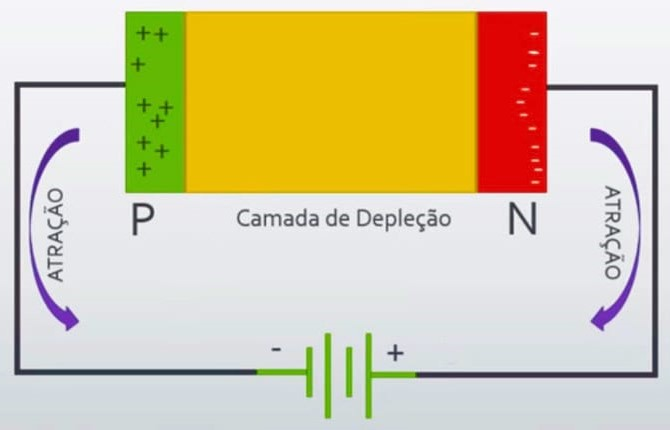
\includegraphics[scale=0.5]{imagens/diodo_polarizado_reversamente.jpg}
			\caption{Diodo polarizado reversamente.}
		\end{figure}
		Em razão da concentração de cargas nos extremos do diodo e do aumento da barreira de potencial, isto é, o aumento da voltagem entre as extremidades da região de depleção, a região de depleção se torna mais larga e podemos pensar nos extremos do diodo como as placas de um capacitor. A junção pn portanto, quando polarizada reversamente, possui capacitância dependente de $V_{R}$.
		
		Uma vez que possui-se o fótodiodo funcionando como um capacitor sob uma tensão reversa, o dispositivo se carregará com um dado valor $V_{C}$ que depende do tempo ao qual o fótodiodo (agora agindo como capacitor) ficou alimentado pela tensão reversa. Com o fótodiodo carregado permite-se a entrada de luz sobre o sensor, que resultará em uma indução de corrente na junção pn e, consequentemente, em uma alteração na tensão $V_{C}$. A partir da observação individual da tensão $V_{C}$ em uma matriz de fótodiodos é possível fazer a transdução da luz incidente sobre o sensor em uma imagem.		
		
\section*{Tipos de sensores de imagem}
		Existem dois principais tipos de sensores de imagem, eles são os CCDs (\textit{Charge-Couple Device}) e os \textit{Active-pixel sensors}, comumente chamados de sensores CMOS. Ambos os dispositivos são feitos com tecnologia MOS (\textit{Metal Oxide Semiconductor}), com CCDs baseados em capacitores MOS e os sensores CMOS baseados em amplificadores MOSFET. A seguir entra-se em mais detalhes sobre cada tipo de sensor, suas características, histórias, vantagens e desvantagens.
		
	\subsection*{A história dos sensores de imagem}
		Apesar dos sensores CCDs terem sido pioneiros no ramo de medição científica nos anos 80 e se tornado o sensor de escolha para praticamente toda aplicação de imagens nesta época, o desenvolvimento de sensores CMOS atingiu um ponto em que começou a substituir os sensores CCDs em aplicações de baixa performance. Com o passar do tempo os sensores de tecnologia CMOS se expandiram, enquanto os de tecnologia CCD estagnaram. 

	
	\subsection*{Sensores CCD}
	Fazer quarta
	\subsection*{Sensores CMOS}
	Fazer quarta
	\subsection*{CCD vs. CMOS}
	Fazer quarta

	\section*{Simulação de um sensor CMOS simplificado}
	Fazer quinta
	\section*{Projeto de um sensor CMOS simplificado}
	Fazer quinta	
	\section*{Extra: Separação de cores}
	Fazer quarta

\end{document}